\documentclass[pdftex,12pt,a4paper]{report}

\usepackage[pdftex]{graphicx}
\usepackage{float}
\usepackage{fancyvrb}
\fvset{xleftmargin=2em}
\usepackage{graphicx}

\usepackage{pgfplots}
\pgfplotsset{width=10cm,compat=1.9}
\usepackage{tikzscale}
\usepackage{pgfplotstable}
\usepackage{booktabs}
\usepackage[font=small,labelfont=bf,tableposition=top]{caption}

\usepackage[utf8]{inputenc} % isto é um comentário
\usepackage[portuges]{babel}
%\usepackage[T1]{fontenc}
\usepackage{times}
%\usepackage{lmodern}
\usepackage[obeyspaces,spaces]{url}
\usepackage[left=25mm,right=25mm,top=25mm,bottom=25mm]{geometry}
\usepackage{titlesec}
\usepackage{mathtools}
%identa 1º paragrafo de capitulos e secções
\usepackage{indentfirst}
\usepackage{graphicx,color}
\newcommand{\HRule}{\rule{\linewidth}{0.5mm}}
\titleformat{\chapter}{\normalfont\huge}{\thechapter.}{20pt}{\huge}


\definecolor{verde}{rgb}{0,1,0}
\definecolor{azul}{rgb}{0,0,1}

\begin{document}

\begin{titlepage}


\begin{minipage}{0.3\textwidth}
\begin{flushleft} 

\includegraphics[width=\textwidth]{logo.png}
\end{flushleft}
\end{minipage}
\begin{minipage}{0.6\textwidth}
\begin{flushright} 

\textsc{Departamento de Engenharia Informática}\\[0.1cm]
\bfseries Mestrado Integrado em Engenharia Informática \\ [0.1cm]
\bfseries \textit{Desenvolvimento Sistemas de Sotware}\\[8mm]

\end{flushright}
\end{minipage}


\vspace{3cm}


\begin{center}


\LARGE System Cost – Partilha de Despesas num Apartamento 
\vspace{3ex}


\LARGE \textbf{1ª Fase }\\[1.5cm]


%{\Large \bfseries Grupo 84\\[2cm] }


\noindent\begin{minipage}[b]{.1\textwidth}
	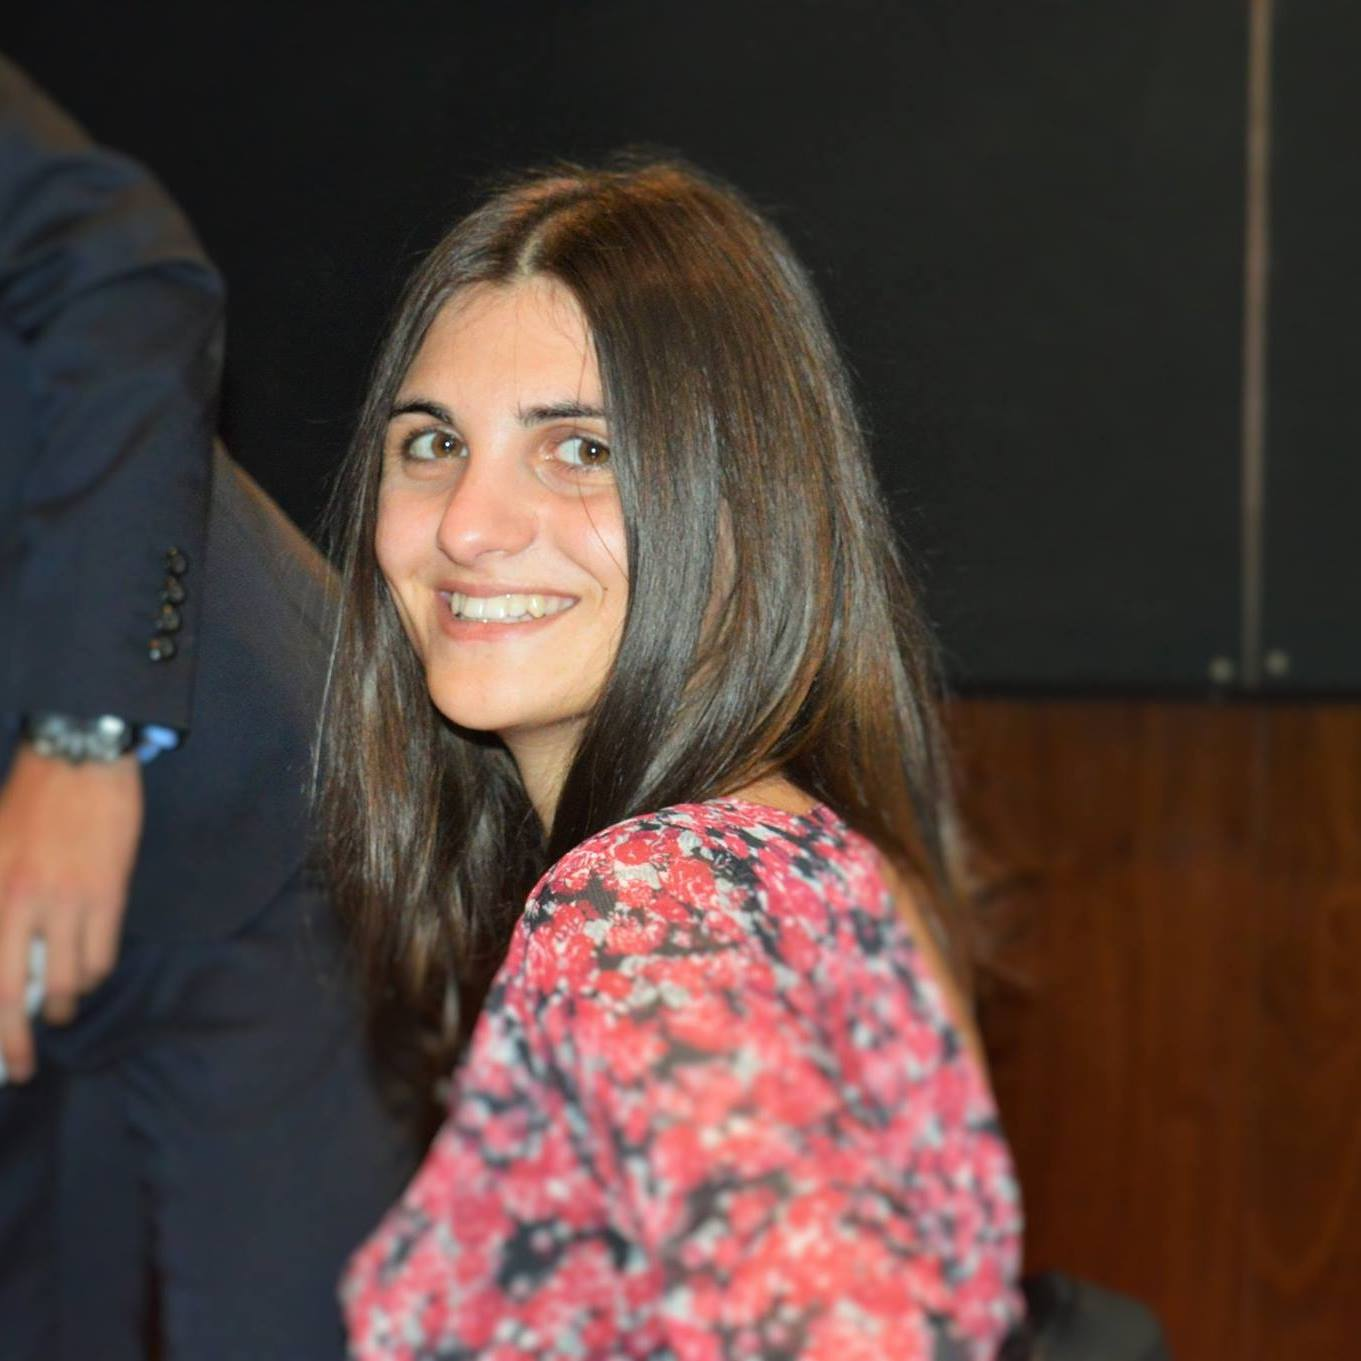
\includegraphics[scale=0.070]{celia}
	\small{Célia Figueiredo a67637}
\end{minipage} 
\hfill
\begin{minipage}[b]{.1\textwidth}
	
\includegraphics[scale=0.36]{gil}
	\small{Gil Gonçalves a67738}
\end{minipage}
\hfill
\begin{minipage}[b]{.1\textwidth}
	
\includegraphics[scale=0.1002]{marcia}
	\small{Márcia Costa a67672}
\end{minipage}
\hfill
\begin{minipage}[b]{.1\textwidth}
	
\includegraphics[scale=0.3]{daniel}
	\small{Daniel Rodrigues a67634}
\end{minipage}
\hfill
\begin{minipage}[b]{.1\textwidth}	
\includegraphics[scale=0.1]{ricardo}
		\small{Ricardo Lopes a72062}
\end{minipage}



\vspace{3ex}


\vfill

\large Braga, {\large \today}

\end{center}
\end{titlepage}

\chapter{Introdução}

No âmbito da unidade curricular de Desenvolvimento de Sistemas de Sotware do 3ºano do curso de MIEI,  foi proposto o desenvolvimento de um projeto que visa a concepção de um sistema que serve de suporte à partilha de despesas num apartamento.

Neste relatório é descrito o processo de análise, modelação e conceção de um sistema que serve de suporte à partilha de despesas num apartamento, foi-nos proposto desenvolver uma aplicação que fosse capaz de fazer o registo das despesas que são geradas num apartamento, assim como a gestão do pagamento feita por cada um dos moradores do apartamento em questão.
Decidimos que seria interessante desenvolver um sistema que permitisse aos utilizadores usufruírem do controlo de terem as suas despesas devidamente divididas, onde os pagamentos das mesmas fossem o mais breve possível, organizado e ainda a facilidade de acesso através de um smartphone, tablet ou pc para a consulta desta mesma aplicação.

O trabalho será dividido em duas fases que se completam uma à outra.
Na primeira fase será descrito o processo de análise de requisitos suportada pelo modelo de domínio do sistema, casos de uso e resptivas especificações e uma possível interface com o utilizador. Tudo isto de forma a enquadrar e descrever da forma mais detalhada possível o sistema a ser desenvolvido. Serão expostos os desenhos de planificação das interfaces e da sua correlação com as funcionalidades a serem implementadas no sistema.
Na segunda fase faremos com que a nossa aplicação ganhe vida e desta forma conseguirmos fazer chegar ao público alvo aquilo que seria o nosso produto final. Desta forma faremos a junção de uma base de dados com o sistema por nós já implementado.

\section{Apresentação do Caso de Estudo}

A aplicação terá como objetivo desenvolver um sistema de despesas num apartamento  capaz de suportar o registo de despesas e a gestão do pagamento dessas mesmas despesas por parte dos moradores. Este é um sistema que proporciona aos seus utilizadores a possibilidade de efetuarem os pagamentos das suas despesas, sejam estas recorrentes (por exemplo, água ou eletricidade) ou extraordinárias (por exemplo, necessidade de realizar alguma reparação no apartamento) fazendo com que o controlo de dívidas entre moradores estejam sempre atualizadas e visíveis para todos os utilizadores da aplicação. 	
Neste sistema existe um morador previamente registado na aplicação necessitando de fornecer o nome, data de nascimento, e-mail e nr de telefone e uma password para efetuar o registo. Terá a ele associada uma conta corrente que será uma espécie de fundo do qual mensalmente (ou quando necessário) é creditado o pagamento, ou seja, a quantia necessária afeta as despesas correspondentes. A conta corrente de cada morador contribui para o saldo global, ou seja, no nosso sistema existe um saldo que resulta do somatório de todas as contas correntes e que corresponde ao montante total que o apartamento tem como despesa nesse mês. 

O saldo global é administrado por um Administrador que é responsável por verificar se o montante deste mesmo está completo e depois dessa forma, pagar a despesa. A todas as despesas está associado um valor assim como cada pagamento creditado da conta corrente de cada morador. 

Ainda de salientar que a cada morador está associada uma fração que varia consoante o tipo de morador (exemplo: moradores que partilham quarto, terão uma fração do valor da renda menor relativamente a um morador com quarto individual), relativamente às restantes despesas (água, luz, gás, internet, ou até mesmo despesas extraordinárias). 


 	

\tableofcontents

\chapter{Requisitos do Sistema}

\section{Análise e Levantamento dos Requisitos}
A aplicação a desenvolver deverá suportar o registo das despesas e a gestão do seu pagamento por parte de moradores registados.

\subsection{Criação do grupo com os elementos da casa/apartamento}

\begin{itemize}
	

\item{Cada morador deve efetuar um registo fornecendo o seu nome, e-mail, número de telemóvel e data de nascimento.}

\item{O morador assim como o utilizador necessitam de efetuar login na aplicação}

\item{O utilizador que convidar os restantes será considerado adminstrador do sistema.} 

\end{itemize}

\subsection{Gestão das contas}

\begin{itemize}
	
\item{Após o registo será associada uma conta corrente a cada utilizador.}

\item{Cada conta corrente permitirá a gestão do saldo corrente (estão incluidas dívidas) de cada morador.}

\item{O morador deverá efetuar um pagamento.}
 
\item{Cada pagamento será creditado na conta corrente do morador.}
 
 \item{O pagamento pode ser igual ou superior à quantia necessária para pagar as despesas em causa.}
 
 
\item{Existirá um saldo global da casa, este que é o somatório de todas as contas correntes dos moradores}
 
 \item{O saldo global é administrado por um Adminstrador}
 
\item{Existem dois tipos de despesas distintos: a despesa recorrente referente a despesas mensais como a água, luz, renda, etc; a despesa extra referente a por exemplo arranjos de material na casa}
 
\item{Cada morador deverá pagar uma fração relativa à despesa}
 
\item{Cada despesa a pagar tem a si associado um tipo (i.e. água, luz, cadeiras, etc)}

\end{itemize}


\section{Base de dados }
A aplicação necessitará de uma implementação de uma base de dados para gerir os elementos que pertencem ao grupo assim como as despesas efetuadas pelos moradores. 

\chapter{Arquitetura da Aplicação}

\section{Modelo de Dominio }
Todo e qualquer projeto possui um domínio específico. O modelo de domínio deve capturar os seguintes pontos: as entidades, os relacionamentos entre as entidades e o vocabulário de domínio do problema. Para além disso também deve ser uma visão estática do problema onde é possível representar as regras de negócio invariantes no tempo. Ou seja, o modelo de domínio é a base para a análise de requisitos.

No que diz respeito à aplicação, como é dito na introdução, queremos desenvolver uma aplicação capaz de suportar o registo das despesas e a gestão do seu pagamento por parte dos moradores registados.


\begin{figure}[htb!]
	\includegraphics[scale=0.4]{imagens/mD/"ModeloDominio"}  
	\caption{Modelo Dominio}  
\end{figure}

O morador necessita de fornecer o nome, e-mail, número de telemovel e data de nascimento, para efetuar o login. 

Como se pode observar na figura o morador efetua pagamento relativo a despesa recorrente ou extra, assim como paga uma fração da despesa, essa fração é relativa a um tipo de despesa. 


O administrador administra o saldo global da casa/apartamento. 


\newpage

\section{Modelo de Use Case}
A segunda parte da análise de requisitos corresponde à definição dos use cases, com o objetivo de os aplicar nesta primeira fase deste trabalho prático. Nos use cases, queremos primeiramente, identificar os atores, que serão quem interagirá com o sistema.
Posterior à identificação dos atores, passamos então à identificação dos use cases, isto é, o que se pretende do sistema. No último ponto da visão orientada aos use cases, procedemos à identificação das classes de suporte à realização dos mesmo, que corresponde à especificação da funcionalidade a ser implementada.
Neste sentido, quando definimos um use case, para além de ser uma espécie de documentação, temos de ter em conta que se trata de uma unidade coerente de funcionalidade, um serviço. Define também um comportamento do sistema, sem revelar a estrutura interna, divulgando desta forma, a comunicação entre os atores e o sistema.
O conjunto de todos os use cases acaba por definir pela íntegra, toda a funcionalidade do sistema que decorre na sua essência, do diálogo entre o sistema e os atores, e a responsabilidade de resposta funcional do sistema.



\subsection{Diagrama de Use Case}


\begin{figure}[htb!]
	\centering
	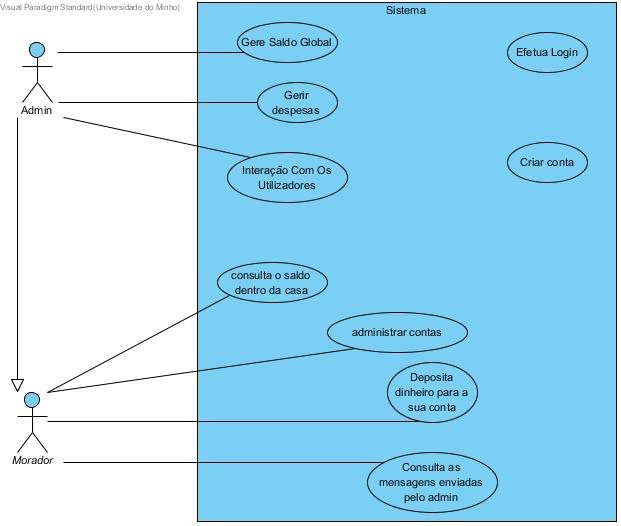
\includegraphics[scale=0.5]{UseCase}  
	\caption{Modelo Use Case}  
\end{figure}

\newpage
\subsubsection{Especificação: Gere Saldo Global }

\begin{figure}[htb!]
	\centering
	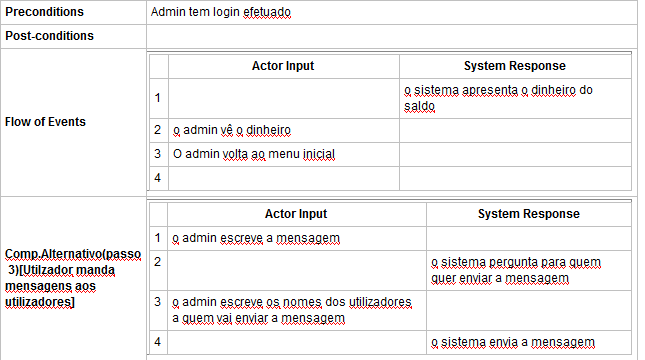
\includegraphics[scale=0.6]{imagens/Especificacoes/geresaldoglobal}  
	\caption{Especificação do Use Case: Gere Saldo Global  }  
\end{figure}


\subsubsection{Especificação: Efetua Login }

\begin{figure}[htb!]
	\centering
	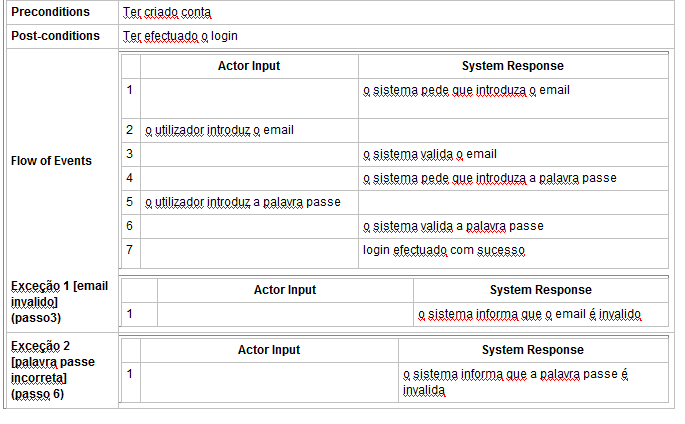
\includegraphics[scale=0.6]{imagens/Especificacoes/efetualogin}  
	\caption{Especificação do Use Case: Efetua Login  }  
\end{figure}

\newpage

\subsubsection{Especificação: Criar Conta }
\begin{figure}[htb!]
	\centering
	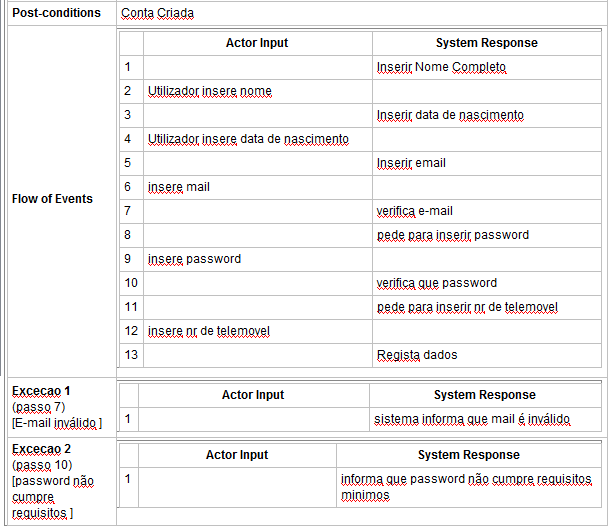
\includegraphics[scale=0.6]{imagens/Especificacoes/criarconta}  
	\caption{Especificação do Use Case: Criar Conta   }  
\end{figure}

\subsubsection{Especificação: Consulta Saldo dentro de casa }
\begin{figure}[htb!]
	\centering
	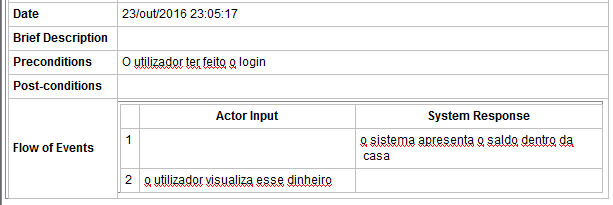
\includegraphics[scale=0.6]{imagens/Especificacoes/consultasaldodentrodecasa}  
	\caption{Especificação do Use Case: Consulta Saldo dentro de Casa   }  
\end{figure}

\newpage

\subsubsection{Especificação: Deposita Dinheiro para a sua Conta }
\begin{figure}[htb!]
	\centering
	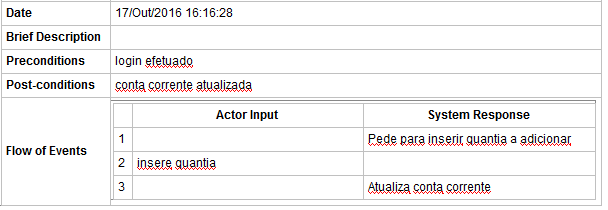
\includegraphics[scale=0.6]{imagens/Especificacoes/depositadinheiro}  
	\caption{Especificação do Use Case: Deposita Dinheiro para a sua conta  }  
\end{figure}

\subsubsection{Especificação: Consulta Mensagens enviadas pelo Administrador }
\begin{figure}[htb!]
	\centering
	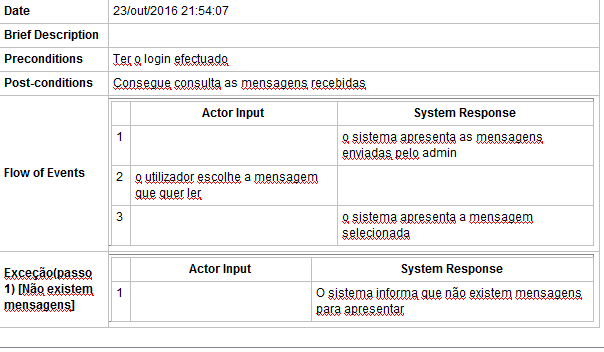
\includegraphics[scale=0.6]{imagens/Especificacoes/consultasmsadmin}  
	\caption{Especificação do Use Case: Consulta Mensagens enviadas pelo Administrador}  
\end{figure}

\newpage
\subsection{Subdiagrama Gerir Despesas}

\begin{figure}[htb!]
	\centering
	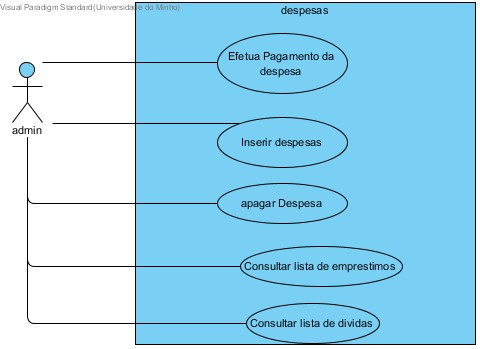
\includegraphics[scale=0.5]{imagens/UseCase/GerirDespesas}  
	\caption{Sub-Diagrama Gerir Despesas }  
\end{figure}

\subsubsection{Especificação: Efetua pagamento da despesa}

\begin{figure}[htb!]
	\centering
	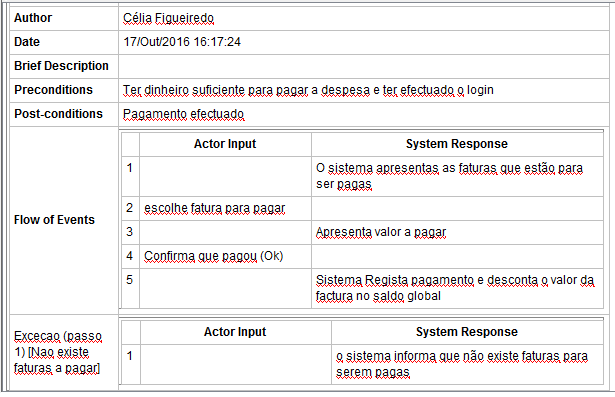
\includegraphics[scale=0.6]{imagens/Especificacoes/efetuapagdespesa}  
	\caption{Especificação do Use Case:Efetua Pagamento da despesa  }  
\end{figure}

\newpage

\subsubsection{Especificação: Inserir Despesa}
\begin{figure}[htb!]
	\centering
	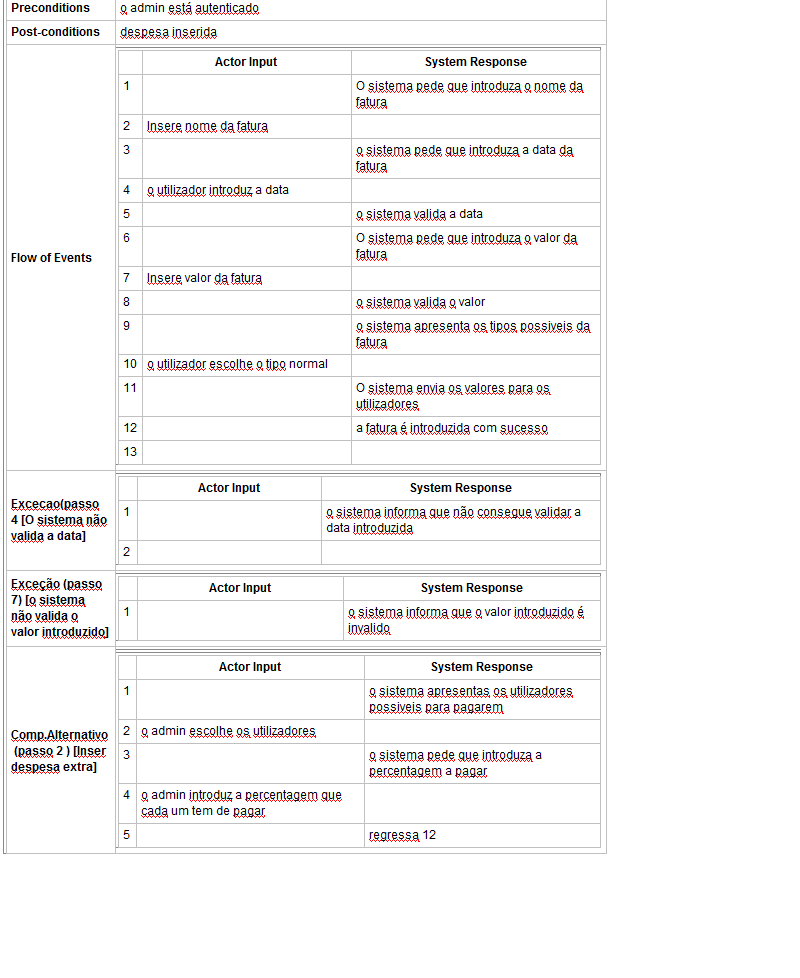
\includegraphics[scale=0.8]{imagens/Especificacoes/inserirdespesas}  
	\caption{Especificação do Use Case: Inserir Despesas}  
\end{figure}

\newpage

\subsubsection{Especificação: Apagar Despesa}

\begin{figure}[htb!]
	\centering
	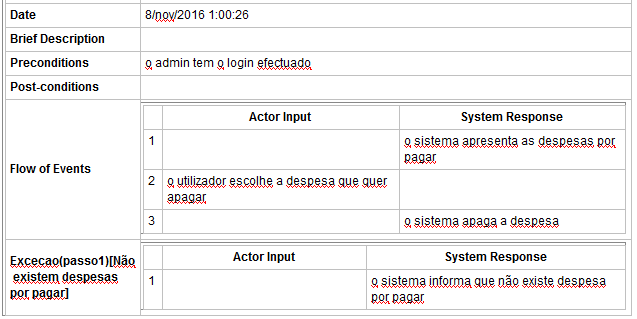
\includegraphics[scale=0.6]{imagens/Especificacoes/apagardespesa}  
	\caption{Especificação do Use Case: Apagar Despesa}  
\end{figure}


\subsection{Subdiagrama Administrar Contas}
\begin{figure}[htb!]
	\centering
	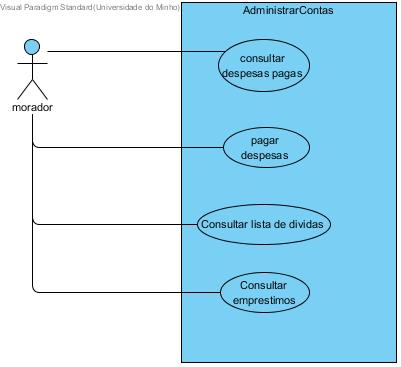
\includegraphics[scale=0.6]{imagens/UseCase/despesasMorador}  
	\caption{Subdiagrama: Administrar Contas }  
\end{figure}

\newpage

\subsubsection{Especificação: Consultar despesas pagas }

\begin{figure}[htb!]
	\centering
	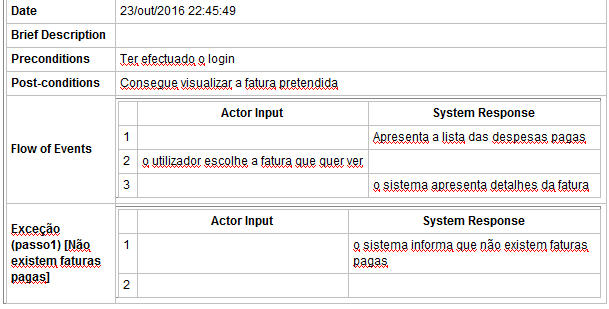
\includegraphics[scale=0.6]{imagens/Especificacoes/consultardespesaspagas}  
	\caption{Especificação do Use Case: Consultar Despesas Pagas}  
\end{figure}

\subsubsection{Especificação: Pagar Despesas }

\begin{figure}[htb!]
	\centering
	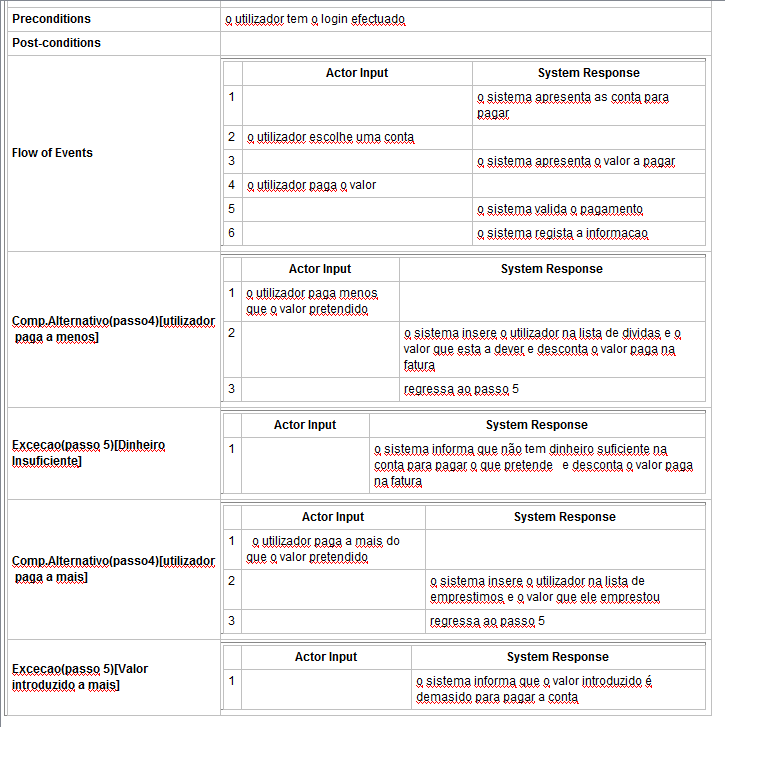
\includegraphics[scale=0.6]{imagens/Especificacoes/pagardespesas}  
	\caption{Especificação do Use Case: Pagar Despesas}  
\end{figure}

\newpage
\subsubsection{Especificação: Consultar Lista de Dívidas }

\begin{figure}[htb!]
	\centering
	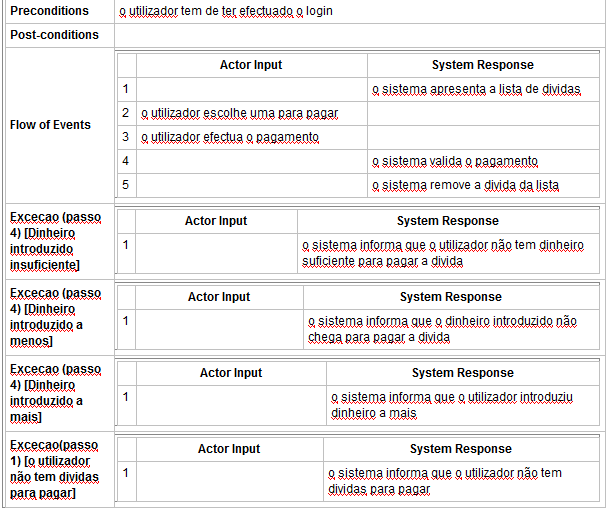
\includegraphics[scale=0.7]{imagens/Especificacoes/consultarlistadedividas}  
	\caption{Especificação do Use Case: Consultar lista de dividas}  
\end{figure}

\subsubsection{Especificação: Consultar Empréstimos }

\begin{figure}[htb!]
	\centering
	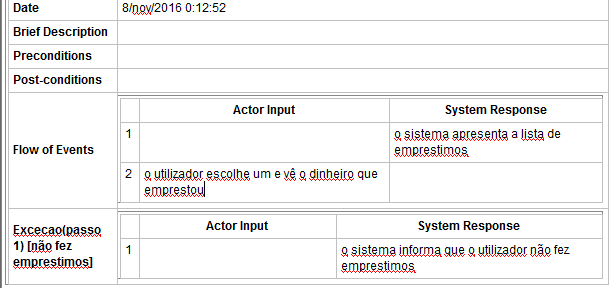
\includegraphics[scale=0.7]{imagens/Especificacoes/consultaremprestimos}  
	\caption{Especificação do Use Case: Consultar Empréstimos}  
\end{figure}

\newpage

\subsection{Subdiagrama Interação com os Utilizadores}
\begin{figure}[htb!]
	\centering
	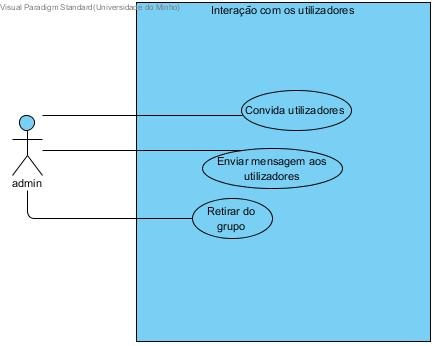
\includegraphics[scale=0.6]{imagens/UseCase/InteracaoComOsUtilizadores}  
	\caption{Subdiagrama: Interação com os utilizadores }  
\end{figure}

\subsubsection{Especificação: Convida Utilizadores }

\begin{figure}[htb!]
	\centering
	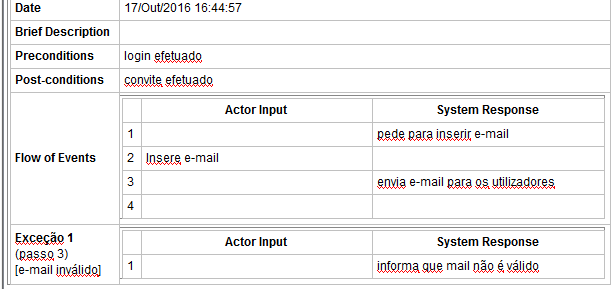
\includegraphics[scale=0.7]{imagens/Especificacoes/convidautilizadores}  
	\caption{Especificação do Use Case: Convida Utilizadores}  
\end{figure}

\newpage

\subsubsection{Especificação: Envia Mensagens aos Utilizadores }

\begin{figure}[htb!]
	\centering
	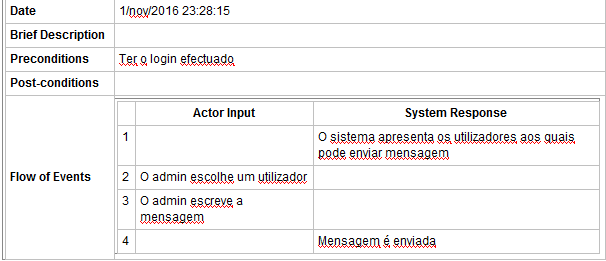
\includegraphics[scale=0.7]{imagens/Especificacoes/enviasmsutilizadores}  
	\caption{Especificação do Use Case: Envia Mensagens aos Utilizadores}  
\end{figure}



\subsubsection{Especificação: Retirar do grupo }

\begin{figure}[htb!]
	\centering
	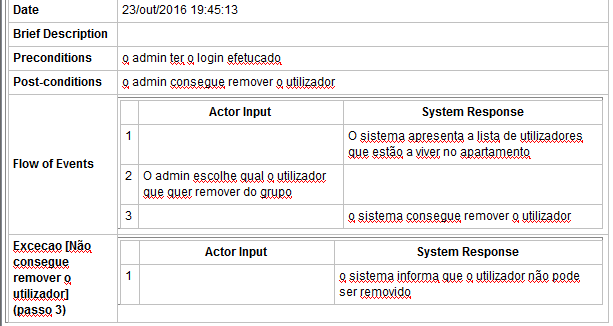
\includegraphics[scale=0.7]{imagens/Especificacoes/retirardogrupo}  
	\caption{Especificação do Use Case: Retirar do grupo}  
\end{figure}

\section{Máquinas de Estado}
\subsection{Efetuar Login}

\begin{figure}[htb!]
	\centering
	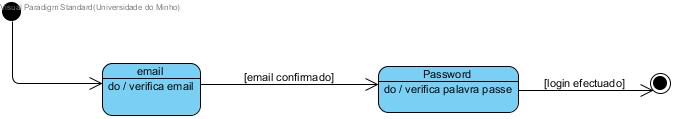
\includegraphics[scale=0.7]{imagens/maqEstados/Login}  
	\caption{Máquina de Estados: Efetuar Login}  
\end{figure}


\subsection{Criar Conta}
\begin{figure}[htb!]
	\centering
	\includegraphics[scale=0.55]{imagens/maqEstados/"Criar Conta"}  
	\caption{Máquina de Estados: Criar Conta}  
\end{figure}

\subsection{Convidar Utilizadores}
\begin{figure}[htb!]
	\centering
	\includegraphics[scale=0.45]{imagens/maqEstados/"Convidar Utilizadores"}  
	\caption{Máquina de Estados: Convidar Utilizadores}  
\end{figure}

\newpage

\subsection{Remover Utilizadores}
\begin{figure}[htb!]
	\centering
	\includegraphics[scale=0.45]{imagens/maqEstados/"Remover Utilizadores"}  
	\caption{Máquina de Estados: Remover Utilizadores}  
\end{figure}

\subsection{Inserir Fatura}
\begin{figure}[htb!]
	\centering
	\includegraphics[scale=0.45]{imagens/maqEstados/"InserFactura"}  
	\caption{Máquina de Estados: Inserir Fatura}  
\end{figure}

\subsection{Deposita Dinheiro}
\begin{figure}[htb!]
	\centering
	\includegraphics[scale=0.45]{imagens/maqEstados/"Deposita Dinheiro"}  
	\caption{Máquina de Estados: Deposita Dinheiro}  
\end{figure}

\newpage
\section{Mockups}
Apresentamos de seguida uma proposta de interface com o utilizador. Utilizámos o programa 'Pencil' para nos auxiliar na construção de uma possivel interface com o utilizador. 


Como já refirmos, para o utilizador efetuar o login necessita de se registar previamente, fornecendo alguns dados que o identifiquem. 
\begin{figure}[htb!]
	\centering
	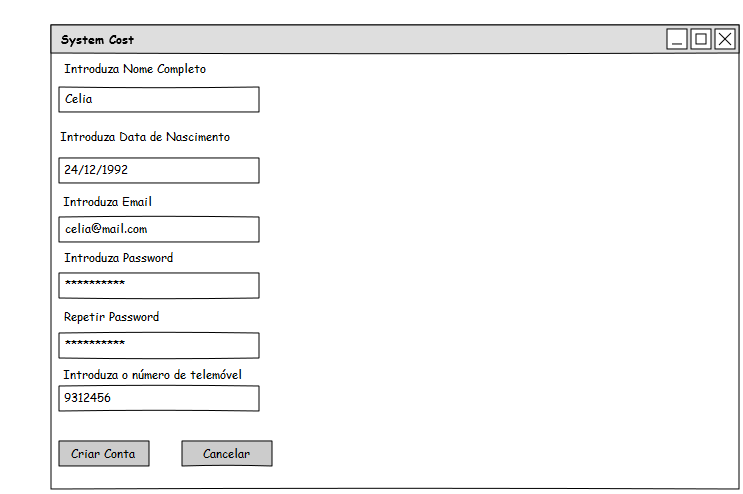
\includegraphics[scale=0.5]{imagens/mockups/CriarConta}  
	\caption{Criar nova Conta }  
\end{figure}

\begin{figure}[htb!]
	\centering
	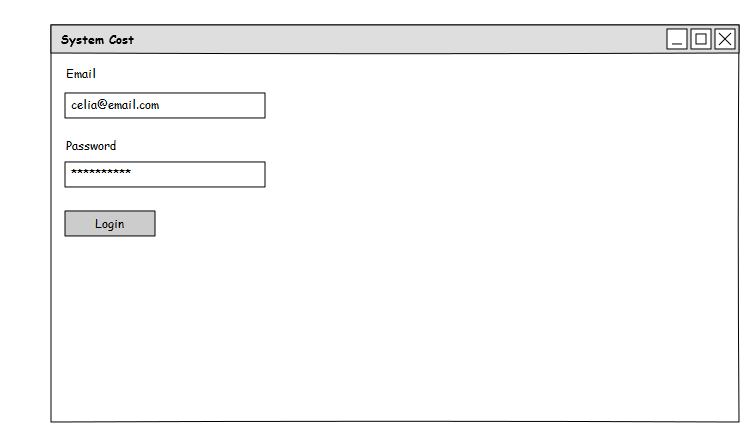
\includegraphics[scale=0.5]{imagens/mockups/MLogin}  
	\caption{Login}  
\end{figure}

\newpage
O Administrador efetua login, mas ainda não existem grupo criado. Pode escolher a opção "Convidar Pessoas", para iniciar a formação de um grupo. 
\begin{figure}[h!]
	\centering
	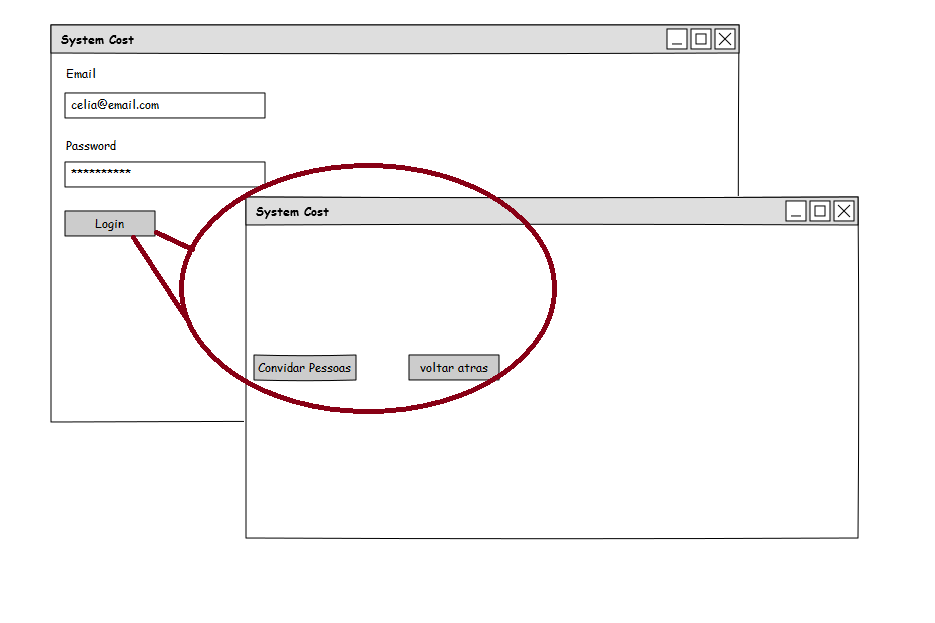
\includegraphics[scale=0.5]{imagens/mockups/loginsemgrupos}  
	\caption{Login quando não existem grupos criados }  
\end{figure}


Haverá sempre a possibilidade de ver/alterar os campos preenchidos inicialmente. 
Carregando no botão grupo abre uma janela onde se pode entrar para grupo constituido pelos elementos da casa/apartamento. Após clicar no botao "Entrar no grupo" é-nos apresentada uma lista com as pessoas já existentes e a possibilidade de convidar mais membros. 

\begin{figure}[htb!]
	\centering
	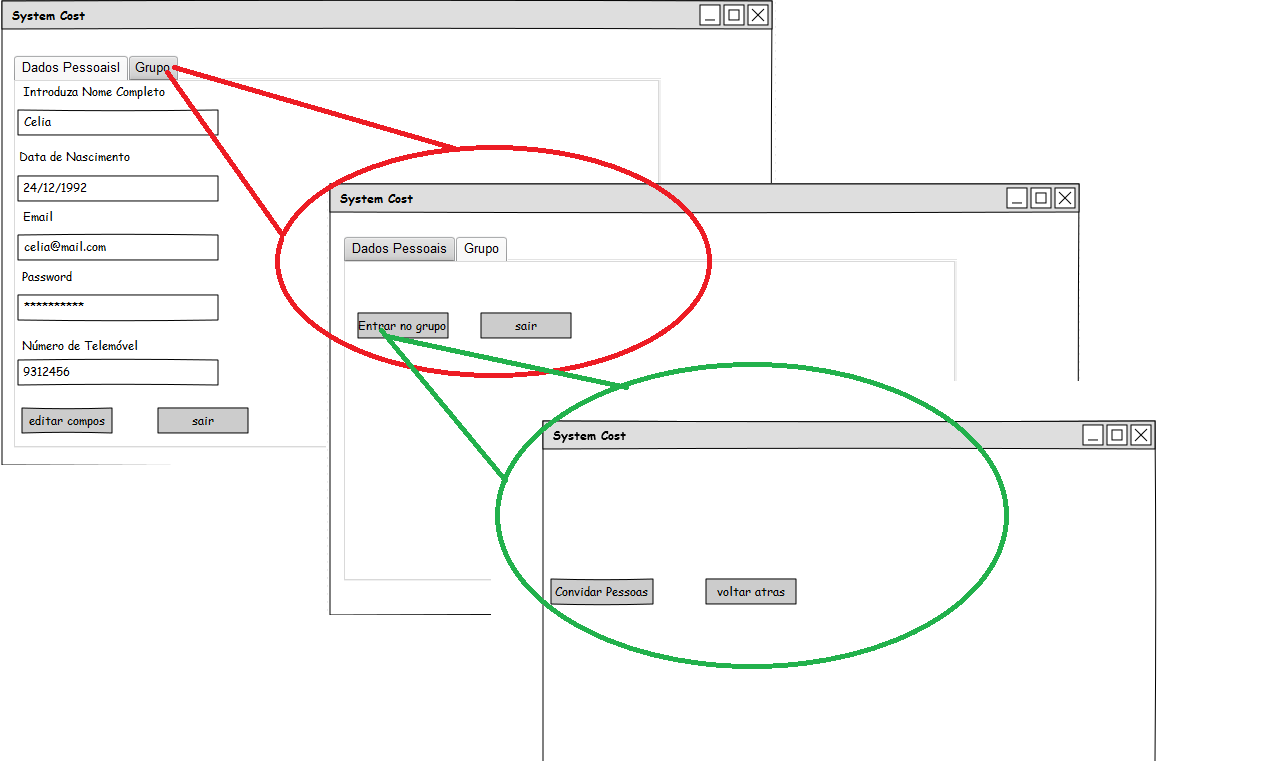
\includegraphics[scale=0.45]{imagens/mockups/consultardados}  
	\caption{Visualização/Alteração dos dados }  
\end{figure}


Após o utililizador efetuar o login é-lhe apresentada uma janela com as funcionalidades que a aplicação lhe oferece, como por exemplo pagar contas e acesso à lista de dividas, assim como o valor da conta corrente. 

\begin{figure}[htb!]
	\centering
	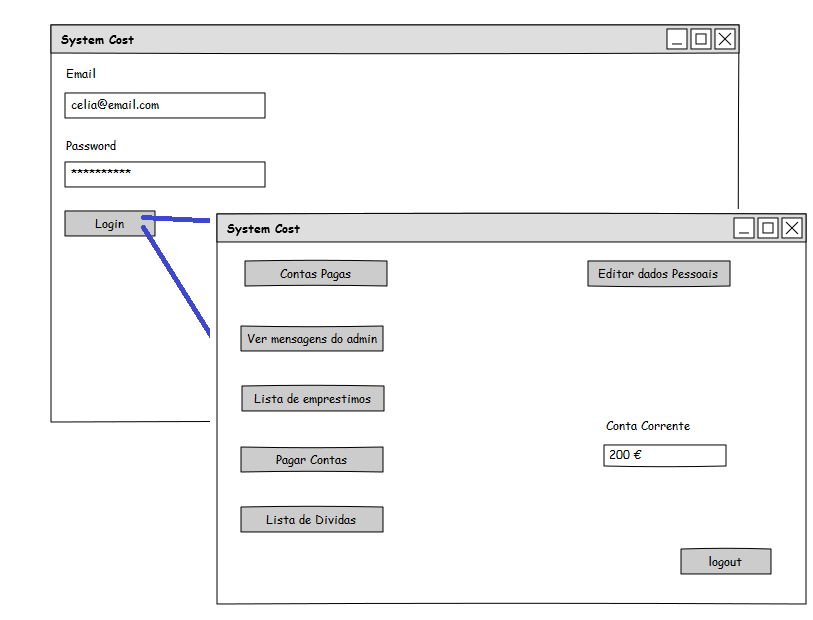
\includegraphics[scale=0.5]{imagens/mockups/logUtilizador}  
	\caption{Login/página inicial }  
\end{figure}

\begin{figure}[h!]
	\centering
	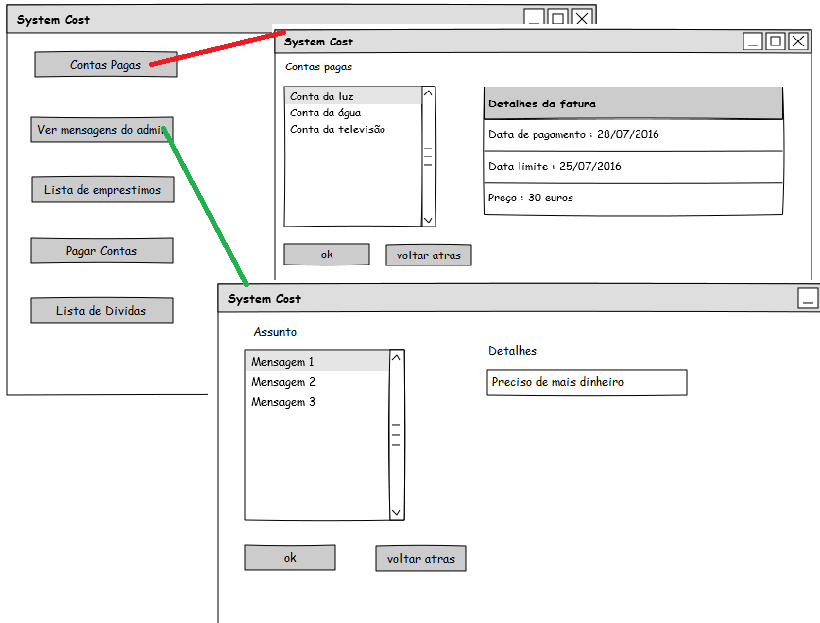
\includegraphics[scale=0.5]{imagens/mockups/tarefasutilizador}  
	\caption{Opções do utilizador }  
\end{figure}

\newpage
Após o administador efetuar o login é-lhe apresentada uma janela com as funcionalidades que a aplicação lhe oferece, como por exemplo pagar contas e adicionar/remover utilizador, enviar mensagem e verificar o saldo global

\begin{figure}[h!]
	\centering
	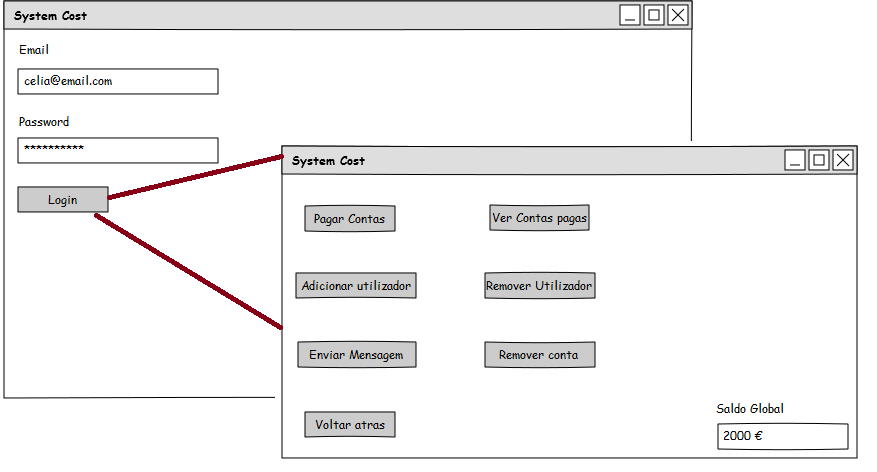
\includegraphics[scale=0.5]{imagens/mockups/loginadmin}  
	\caption{Login/Privilégios de administrador }  
\end{figure}













\chapter{Conclusão}

Para concluir esta primeira fase de modelação do projeto que consiste em  desenvolver um sistema de suporte à partilha de despesas num apartamento, foi-nos proposto enquadrar e descrever da forma mais detalhada possível o sistema a ser desenvolvido. Para isso fizemos uma descrição do processo de análise de requisitos construindo assim o modelo de domínio.  Do modelo de domínio e requisitos do sistema foi possível desenvolver os diagramas de 'Use Case' e a posterior especificação de cada um deles. 

Depois de todos estes elementos procedemos à fase de pensar de como seria a nossa aplicação fisicamente falando e então para tal utilizamos o programa 'Pencil' e desta forma desenvolvemos a nossa primeira proposta de interface com o utilizador. Construimos também os diagramas de máquinas de estado de acordo com a interface pensada. Porém estes dois pontos ainda têm muitas arestas para limar, pois ainda não temos uma interface completa com todas as possiveis funcionalidades. 

Um dos principais problemas que encontramos foi a modelação do Modelo de Dominio, pois estavam sempre a surgir novos requisitos e a serem eliminados outros assim como nas especificações dos 'Use Case'. Podemos concluir que esta é uma etapa que requer uma análise muito cuidada, pois estão sempre a surgir novas maneiras de abordar o projeto. 


Para a fase final do projeto desenvolvemos os "Diagramas de Sequência" com o objetivo de descrever o funcionamento da aplicação e percebemos que alguns "use cases" precisavam de ser alterados.  Depois de muita discussão e partilha de ideias concebemos a aplicação com o objetivo de ser eficiente e simples de usar, com uma interface apelativa. 
A solução usada para o problema pareceu-nos a melhor e fácil de implementar, contudo esta solução está dependente da seriedade dos moradores da casa, por exemplo quando um morador empresta dinheiro poderá nunca o vir a receber. 
Em relação a trabalho futuro fica implementar um sistema que permita a troca de mensagens entre os utilizadores e não só o administrador a enviar mensagens, o administrador saber que aquela mensagem foi vista por todos , ou quantos ainda não vieram essa mensagem, de maneira a que o admin saiba quem viu ou não a mensagem e consequentemente poder apagá-la. 
Outro aspeto a melhorar é o caso de o utilizador emprestar dinheiro ao utilizador diretamente da conta dele. 
Na apresentação das contas/mensagens o utilizador primeiro vê as mensagens e só quando carregar é que consegui ver o detalhe das mesmas. 
Aplicação foi submetida a testes, e  corrigida quando os testes falhavam no entanto há sempre testes que não conseguimos até ao momento prever. 






\end {document}


